\documentclass[12pt]{article}

\usepackage{amsmath, amsthm, amssymb, amsbsy, amsfonts}
\usepackage[plainpages=false,pdfpagelabels]{hyperref}
\hypersetup{
    colorlinks,
    citecolor=black,
    filecolor=black,
    linkcolor=black,
    urlcolor=blue
}
\usepackage{verbatim}
\usepackage{enumitem}
\usepackage[utf8x]{inputenc}

% Redefine the \vec command to use bold font instead of an arrow
\renewcommand\vec[1]{\mathbf{#1}}

%\def\nl{\hfill\break\null}
\oddsidemargin=0.3cm
\topmargin=-1cm
\textwidth=15cm
\textheight=23cm
\parindent=0cm
\parskip=1mm


\usepackage{graphicx}
\DeclareMathOperator*{\argmin}{argmin}

\newenvironment{enumialpha}{\begin{enumerate}
  \def\theenumi{\alph{enumi}}
  \def\labelenumi{(\theenumi)}}{\end{enumerate}}

\newenvironment{enumiiroman}{\begin{enumerate}
  \def\theenumii{\roman{enumii}}
  \def\labelenumii{(\theenumii)}}{\end{enumerate}}


\begin{document}

\begin{tabular*}{15cm}{@{}l@{\extracolsep{\fill}}r}
  Albert-Ludwigs-Universit\"at Freiburg, Institut f\"ur Informatik \\
PD Dr. Cyrill Stachniss \\  Lecture: Robot Mapping \\
  Winter term 2013 
\end{tabular*}

\bigskip


\begin{center}
{\bf \Large Sheet 6}

{\large Topic: Unscented Kalman Fitler SLAM}

Submission deadline: Dec.~9\\
Submit to: \texttt{robotmappingtutors@informatik.uni-freiburg.de}
\end{center}

\subsubsection*{Exercise: UKF SLAM}

Implement an unscented Kalman filter SLAM~(UKF SLAM) system. You should
complete the following parts:

\begin{enumialpha}

  % rk: I give them the implementation to avoid failures when using chol or
  % sqrtm. Furthermore, unscented transform was covered on Sheet 5
%\item Implement the function in \texttt{compute\_sigma\_points.m},
  %which samples sigma points given a mean vector and
  %covariance matrix according to the unscented transform.

\item Implement the prediction step of the filter by completing the
  function in \texttt{prediction\_step.m} to compute the mean and
  covariance after incorporating the odometry motion command.

\item Implement the correction step in \texttt{correction\_step.m} to
  update the belief after each sensor measurement according to the UKF
  SLAM algorithm.

\end{enumialpha}

To support this task, we provide a small \emph{Octave} framework (see
course website). The above-mentioned tasks should be implemented inside
the framework in the directory \texttt{octave} by completing the stubs.
After implementing the missing parts, you can test your solution by
running the script in \texttt{ukf\_slam.m}. The program will produce
plots of the robot pose and map estimates and save them in the
\texttt{plots} directory. Figure~\ref{fig:ukfStates} depicts some
example images of the state of the UKF.

Note that, as opposed to the EKF SLAM system you implemented in sheet 4,
here the state vector and covariance matrix are incrementally grown with
each newly-observed landmark. The mean estimates of the landmark poses
are stacked in $\mu_t$ in the order by which they were observed by the
robot, as described in the \emph{map} vector in the framework.

Some implementation tips:
\begin{itemize}
  \item
    Be careful when averaging angles. One way to average a set of angles
    $\left\{ \theta_1, \ldots, \theta_N \right\}$ given their weights
    $\left\{ w_1, \ldots, w_N \right\}$ is to first compute the weighted
    sum of the unit-vectors of each rotation
    \begin{eqnarray*}
      \bar x = \sum_{i=1}^N w_i \cos(\theta_i),\quad\quad
      \bar y = \sum_{i=1}^N w_i \sin(\theta_i).
    \end{eqnarray*}
    Then the average angle $\bar \theta$ is given by
    \begin{equation*}
      \bar \theta = \mathrm{atan2}(\bar y, \bar x).
    \end{equation*}
  \item Remember to normalize the angles after you computed a sum or a
    difference involving angles.
  \item Turn off the visualization to speed up the computation by
    commenting out the line \texttt{plot\_state(...)} in the file
    \texttt{ukf\_slam.m}.
  \item While debugging, run the filter only for a few steps by
    replacing the for-loop in \texttt{ukf\_slam.m} by something along
    the lines of \texttt{for t = 1:50}.
  \item The command \texttt{repmat} allows you to replicate a given
    matrix in many different ways and is magnitudes faster than using
    for-loops.
  \item When converting implementations containing for-loops into a
    vectorized form it often helps to draw the dimensions of the data
    involved on a sheet of paper.
  \item Many of the functions in \emph{Octave} can handle matrices and
    compute values along the rows or columns of a matrix. Some useful
    functions that support this are \texttt{sum}, \texttt{sqrt},
    \texttt{sin}, \texttt{cos}, and many others.
\end{itemize}

\begin{figure}
  \centering
  \begin{tabular}{@{}c@{\hspace{2mm}}c@{\hspace{2mm}}c@{}}
    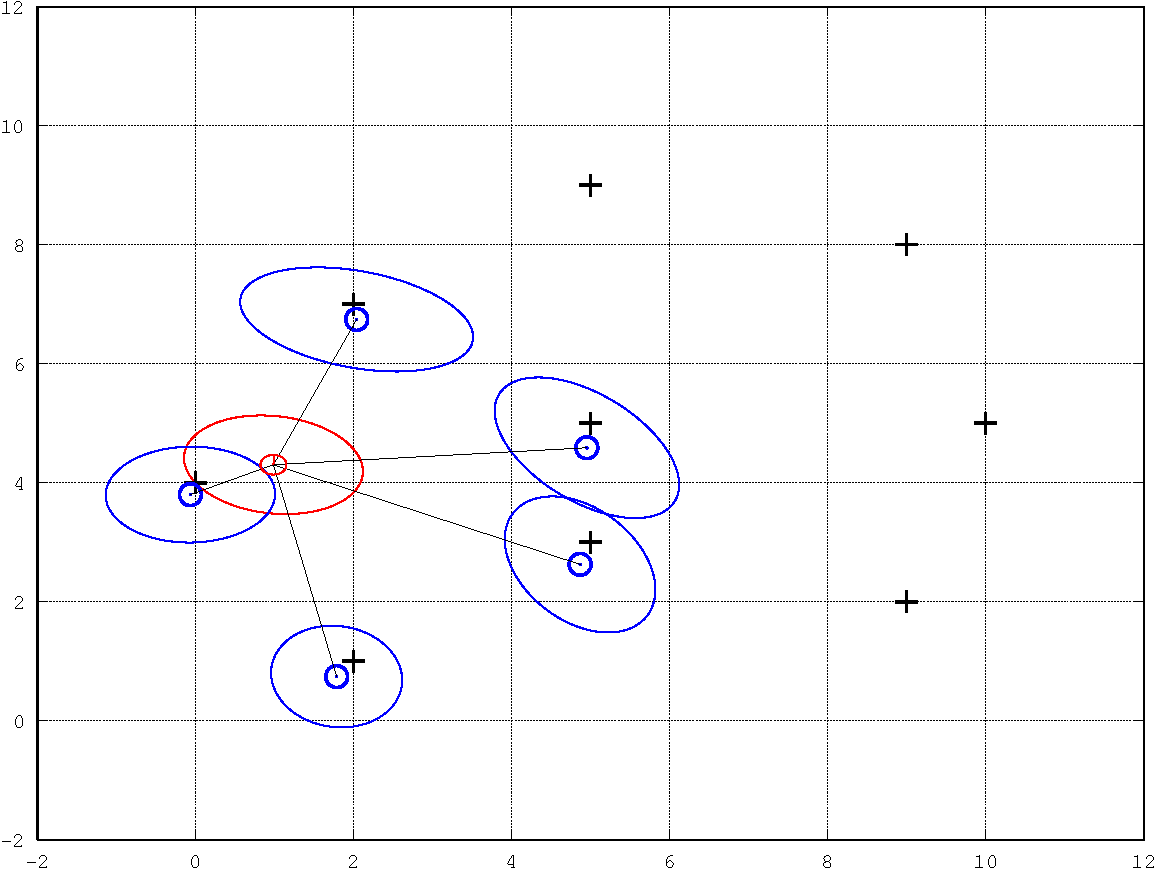
\includegraphics[width=0.32\columnwidth]{ukf_050} &
    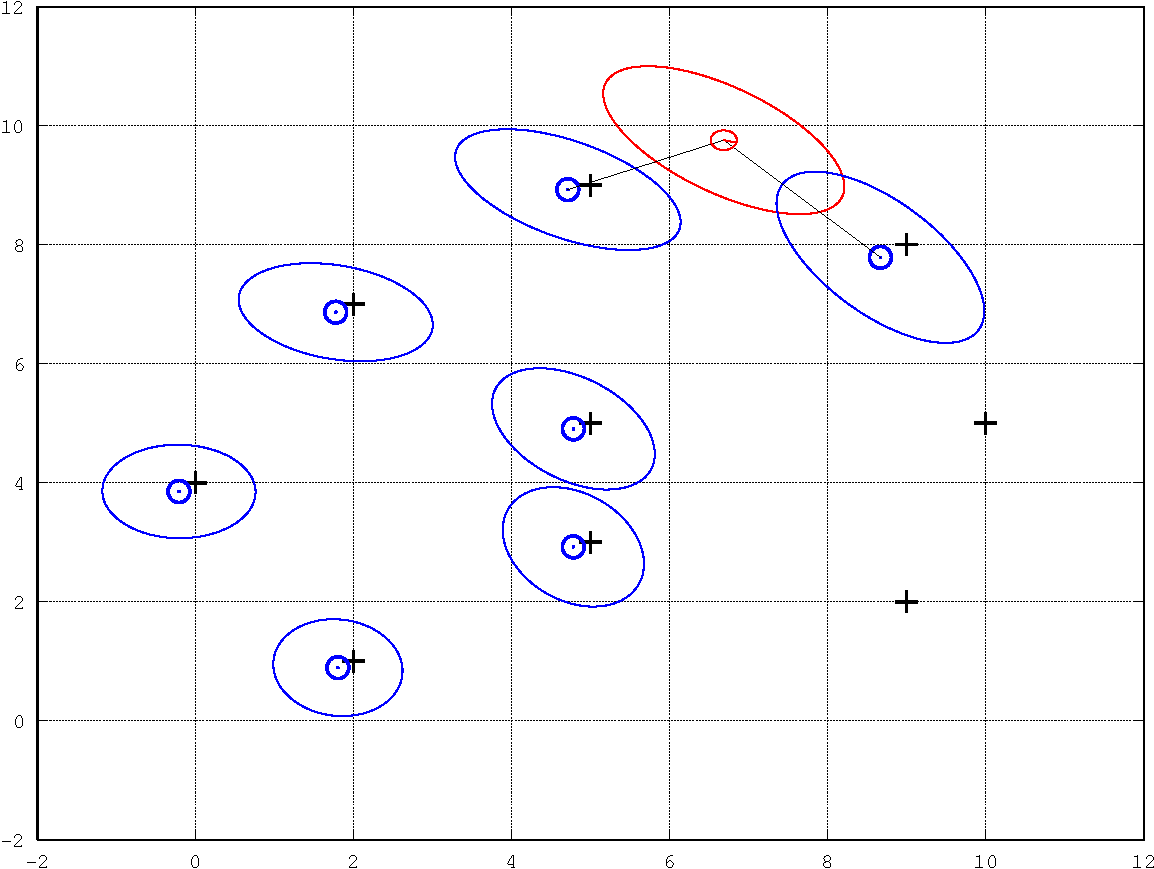
\includegraphics[width=0.32\columnwidth]{ukf_150} &
    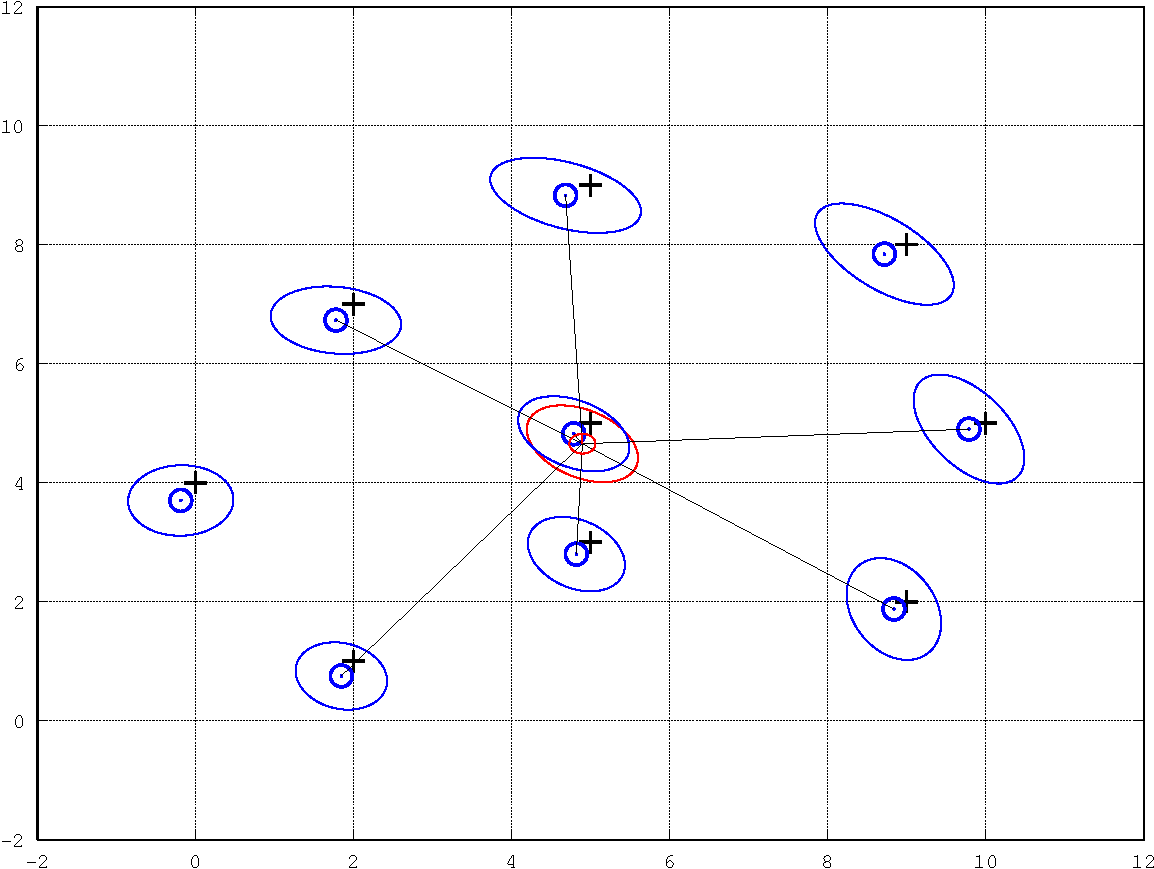
\includegraphics[width=0.32\columnwidth]{ukf_330} \\
    $t=50$ & $t=150$ & $t=330$
  \end{tabular}
  \caption{Example images of the state of the UKF at certain time
  indices.}
  \label{fig:ukfStates}
\end{figure}

\end{document}

